% siminos/presentations/kittens/Hill.tex        pdflatex Hill; biber Hill
% $Author: predrag $ $Date: 2021-06-25 01:34:54 -0400 (Fri, 25 Jun 2021) $

% when you get      LaTeX Error: Command \block already defined.
%                   l.512 \newcommand{\block}[1]{\ensuremath{#1}}
% press [Enter] once

% kittens.tex had been split into                                          2020-09-25
%    Bernoulli.tex   Bernoulli.mp4
%    templatt.tex    templatt.mp4
%    catlatt.tex     catlatt.mp4
%    Hill.tex
% EDIT those, not this kittens.tex

                        \newif\ifboyscout\boyscouttrue          %% comments     %%
                        \newif\ifsubmission\submissionfalse     %% internal     %%
                        \newif\ifblog\blogfalse %% section shared with blogCats %%

\input ../../inputs/layoutBeamer
\usepackage[font=scriptsize, labelfont=bf]{caption}
\usepackage[
    backend=biber,  %bibtex,
    sorting=nyt,
    %refsection=chapter,
    %citereset=chapter,
    style=numeric, %alphabetic, % %style=authoryear,
    natbib=true,
    style=phys, % aps
    biblabel= brackets, % superscript, %
    articletitle=false, % true,  % false, % aps
    %chaptertitle=true,  % aip;  % false, % aps
    pageranges = true , % aip: the full range
             % = false, % aps: only the first page being printed
    sortlocale=en_US,
    firstinits=true,
    url=false, %true,  %
    doi=false, %true,
    eprint=false
]{biblatex}
\addbibresource{../../bibtex/siminos.bib}
\setbeamerfont{footnote}{size=\tiny}
%\input ../../inputs/def % no edits, always from dasbuch/book/inputs
\input defsKittens
\input ../../inputs/defsBeamer
\renewcommand{\Ssym}[1]{{\ensuremath{m_{#1}}}}    % Boris
% \newcommand{\Ssym}[1]{{\ensuremath{s_{#1}}}}  % ChaosBook
% \newcommand{\D}{\mathcal{D}}
% \newcommand{\gd}{\mathsf{g}}

\begin{document}
\title{
{\huge \HillDet} %\catlatt}
    \\
{cat in $1$ spacetime dimension}
}
\author{P. Cvitanovi\'c}
\author[Cvitanovi\'c]
{
  \textcolor{green!50!black}{
  {Predrag~Cvitanovi\'c
   and
   Han Liang
%   \\
%  Matt Gudorf,
  }	%\inst{1}
  }
}
\institute
{
%  \inst{1}%
%\HREF{https://itsatcuny.org/calendar/chaos-and-quantum-field-theory}
%{ITS Symposium on Chaos and Quantum Field Theory}
 ChaosBook.org/overheads/spatiotemporal/kittens/   ~ notes
 \\
               Georgia Tech
 }
\date{June 25, 2021}

%\begin{frame}{} %herding cats}
%\begin{center}
%\hfill
\includegraphics[width=0.95\textheight]{DawnBishopCats}
%\end{center}
%\end{frame}

\renewcommand{\statesp}{phase space}

\begin{frame}{a fair dice throw}
    \begin{block}{slope ${6}$ Bernoulli map}
\begin{center}
            \begin{minipage}[c]{0.32\textwidth}\begin{center}
% ChaosBook {fig:BernPartExam}
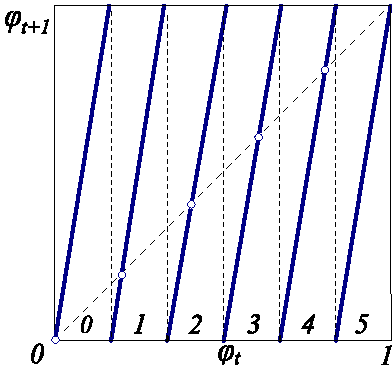
\includegraphics[width=1.0\textwidth]{fig_d_2kitten} % {fig_d_2CL18}
            \end{center}\end{minipage}
            \hspace{2ex}
            \begin{minipage}[c]{0.46\textwidth}
\(
\ssp_{\zeit+1}
= {6} \ssp_{\zeit} - \Ssym{\zeit+1}
\,,\;  \ssp_{\zeit}\in\pS_{\Ssym{\zeit}}
\)
\medskip

${6}$-letter alphabet \\
\(
\Ssym{\zeit} \in \A=\{0,1,2,\cdots,5\}
\)
            \end{minipage}
\end{center}
$6$ subintervals $\{\pS_{0},\pS_{1},\cdots,\pS_{5}\}$
    \end{block}
\end{frame} %%%%%%%%%%%%%%%%%%%%%%%%%%%%%%%%%%%%%%%%%%%%%%

\begin{frame}{what is ({mod}\;1) ?}
\renewcommand{\ssp}{\ensuremath{x}}             % lattice site field
map with integer-valued {\color{blue}`stretching' parameter $s>1$} :
\[
\ssp_{\zeit+1} \,=\, {s}\,\ssp_{\zeit}
\] %ee{BerStretch}

$(\mbox{mod}\;1)$ :
subtract the integer part
\(
\Ssym{\zeit+1}=\left\lfloor{s}\ssp_{\zeit}\right\rfloor
\)

\renewcommand{\ssp}{\ensuremath{\phi}}             % lattice site field
so fractional part
$\ssp_{\zeit+1}$ stays in the unit interval $[0,1)$
\[
\ssp_{\zeit+1}
= {s} \ssp_{\zeit} - \Ssym{\zeit+1}
\,,\qquad  \ssp_{\zeit}\in\pS_{\Ssym{\zeit}}
\] %ee{circ-m}
$\Ssym{\zeit}$ takes values in the ${s}$-letter alphabet
\[
\Ssym{} \in \A=\{0,1,2,\cdots,s-1\}
\] %ee{base-sAlph}
\end{frame} %%%%%%%%%%%%%%%%%%%%%%%%%%%%%%%%%%%%%%%%%%%%%%

\begin{frame}{lattice Bernoulli}
recast the time-evolution Bernoulli map
\[
\ssp_{\zeit+1}
= {s} \ssp_{\zeit} - \Ssym{\zeit+1}
\] %ee{circ-m}
as 1-step difference equation on the {\color{blue}temporal lattice}
\beq
\ssp_{\zeit} - {s}\ssp_{\zeit-1} = - \Ssym{\zeit}
\,,\qquad  \ssp_{\zeit} \in [0,1)
\ee{1stepDiffEq}
{\color{blue}field} $\ssp_\zeit$, {\color{blue}source} $\Ssym{\zeit}$ \\
on each site $\zeit$ of a
1\dmn\ lattice $\zeit\in\integers$
\bigskip

 write an \cl{}-sites lattice segment as \\
the {\color{blue}lattice state} and the {\color{blue}symbol \brick}
\beq
{\Xx} % = \{\ssp_j\}
             = (\ssp_{\zeit+1},\cdots,\ssp_{\zeit+\cl{}})
\,,\quad
{\Mm} % = \{\Ssym{j}\}
             = (\Ssym{{\zeit+1}},\cdots,\Ssym{{\zeit+\cl{}}})
\ee{pathBern}
`$\Mm$' for `marching orders' ~~:~~ come here, then go there, $\cdots$
\end{frame} %%%%%%%%%%%%%%%%%%%%%%%%%%%%%%%%%%%%%%%%%%%%%%

\begin{frame}{think globally, act locally}
Bernoulli {\color{blue}condition} at every lattice site $\zeit$,
{\color{blue}local} in time
\beq
\ssp_{\zeit} - {s}\ssp_{\zeit-1} = - \Ssym{\zeit}
\ee{1stepDiffEq}
is enforced by the {\color{blue}global} equation
\[
\jMorb\Xx+\Mm =0
\,,
\]
where $\jMorb$ is $[\cl{}\!\times\!\cl{}]$ {\color{blue}Hill matrix}
({\jacobianOrb})
\beq
\jMorb
=  \left(\begin{array}{ccccc}
             1    &  0    &        &   & -s\cr
            -s    &  1    &   0    &   &  \cr
                  & -s    &   1    & \ddots &  \cr
                  &       &  -s    & 1 & 0 \cr
             0    &       &        &-s & 1
          \end{array} \right)
\ee{hopMatrix}
\end{frame} %%%%%%%%%%%%%%%%%%%%%%%%%%%%%%%%%%%%%%%%%%%%%%

\begin{frame}{think globally, act locally}
solving the {lattice Bernoulli} system
\[
\jMorb\Xx+\Mm =0
\,,
\]
is a search for zeros of the function
\beq
F[\Xx] = \jMorb\Xx+\Mm = 0
\ee{tempFixPoint}
the entire {\color{blue}global lattice state} ${\Xx}_{\Mm}$ is now
\medskip

a single {\color{blue}fixed point}
$(\ssp_1,\ssp_{2},\cdots,\ssp_{\cl{}})$

\hfill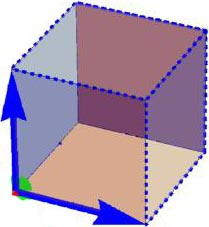
\includegraphics[width=0.12\textwidth]{hyperCube}

\hfill
in the \cl{}\dmn\ unit hyper-cube ~~~~~~~~~~~$\Xx\in[0,1)^\cl{}$
\end{frame} %%%%%%%%%%%%%%%%%%%%%%%%%%%%%%%%%%%%%%%%%%%%%%

\begin{frame}{what does this global \jacobianOrb\ do?}
    \begin{block}{$[\cl{}\!\times\!\cl{}]$ \jacobianOrb}
\[
\jMorb_{ij} =\frac{\delta F[\Xx]_i}{\delta \ssp_j}
\] %ee{jacobianOrb}
    \end{block}
\vfill
\begin{itemize}
              \item
global stability of lattice state \Xx, perturbed everywhere
            \end{itemize}
\end{frame} %%%%%%%%%%%%%%%%%%%%%%%%%%%%%%%%%%%%%%%%%%%%%%

\begin{frame}{next : we derive Hill's formula}
\begin{block}{\jacobianOrb}
\(
\jMorb_{ij} =\frac{\delta F[\Xx]_i}{\delta \ssp_j}
\)
stability under {\color{blue}global} perturbation of the whole orbit

\hfill for \cl{} large, a huge $[d\cl{}\!\times\!d\cl{}]$ matrix
\end{block}
\begin{block}{temporal {\jacobianM}}
\(
\jMps%_\Mm
\)
propagates {\color{blue}initial} perturbation $\cl{}$ time steps

\hfill small $[d\!\times\!d]$ matrix
\end{block}
\vfill

$\jMps$ and $\jMorb$ are related by\footfullcite{Hill86}
\begin{block}{Hill's 1886 remarkable formula}
\[
|\Det\jMorb_\Mm| = |\det(\matId - \jMps_\Mm)|
%\label{catHillform}
\]
\end{block}
$\jMorb$ is {\color{red}huge}, even $\infty$\dmn\ matrix\\
$\jMps$ is {\color{red}tiny}, few degrees of freedom matrix
\end{frame} %%%%%%%%%%%%%%%%%%%%%%%%%%%%%%%%%%%%%%%%%%%%%%

\begin{frame}{temporal stability}
any discrete time dynamical system :
an $\cl{}$-periodic lattice state $\Xx_p$
satisfies the first-order difference equation
\beq
\ssp_{\zeit} - \flow{}{\ssp_{\zeit-1}} = 0
    \,,\quad
\zeit=1,2,\cdots,\cl{}
\,.
\ee{1stepNonlimTemp}
A deviation $\Delta\Xx$ from $\Xx_p$ satisfies the linear equation
\beq
\Delta\ssp_{\zeit} - \jMat_{\zeit-1}\,\Delta\ssp_{\zeit-1} = 0
\,,\qquad
(\jMat_{\zeit})_{ij}
=
\left.\frac{\partial \flow{}{\ssp}_i}
           {\partial \ssp_{j}}\right|_{\ssp_{j}=\ssp_{\zeit,j}}
\,,
\ee{d-1stepJac2}
where $\jMat_{\zeit}$ is the 1-time step $[d\!\times\!{d}]$
\jacobianM.
\end{frame} %%%%%%%%%%%%%%%%%%%%%%%%%%%%%%%%%%%%%%%%%%%%%%

\begin{frame}{temporal period $\cl{}=3$ example}
in terms of the $[3d\!\times\!3d]$
shift matrix $\hopMat$, the \jacobianOrb\
takes block matrix form
\beq
\jMorb_p \,=\,
\id - \hopMat^{-1} \jMat
\,,\quad
\hopMat^{-1} =
\left[
\begin{array}{ccc}
0     & 0     & \id_d  \\
\id_d & 0     & 0  \\
0     & \id_d & 0
\end{array}
\right]
\,,\quad
\jMat =
\left[
\begin{array}{ccc}
\jMat_1 & 0 & 0 \\
0 & \jMat_2 & 0  \\
0 & 0 & \jMat_3
\end{array}
\right]
\,,
\ee{3shift}
where $\id_d$ is the $d$-\dmn\ identity matrix
\medskip

the third repeat of $\hopMat^{-1}\jMat$ is block-diagonal
\bea
(\hopMat^{-1}\jMat)^2 &=&
\hopMat^{-2}
\left[
\begin{array}{ccc}
\jMat_2\jMat_1 & 0 & 0 \\
0 & \jMat_3 \jMat_2 & 0  \\
0 & 0 & \jMat_1\jMat_3
\end{array}
\right]
\continue
(\hopMat^{-1}\jMat)^3  &=&
\left[
\begin{array}{ccc}
\jMat_2\jMat_1\jMat_3 & 0 & 0 \\
0 & \jMat_3\jMat_2\jMat_1 & 0  \\
0 & 0 & \jMat_1\jMat_3\jMat_2
\end{array}
\right]
\quad \mbox{ as } \hopMat^{3}=\id
\nnu %\label{stabSquare}
\eea
\end{frame} %%%%%%%%%%%%%%%%%%%%%%%%%%%%%%%%%%%%%%%%%%%%%%

\begin{frame}{period \cl{} temporal stability}
as $\hopMat^\cl{}=\id$, the trace of the
$[\cl{}d\!\times\!\cl{}d]$ matrix for a period $\cl{}$ lattice state
\[
\Tr(\hopMat^{-1}\jMat)^k=\delta_{k,r\cl{}}\,\cl{}\,\tr\jMat_p^r
\,,\quad
\jMat_p = \jMat_\cl{}\jMat_{\cl{}-1}\cdots\jMat_2\jMat_1
\]
non-vanishing only if $k$ is a multiple of $\cl{}$, where $\jMat_p$ is the
forward-in-time $[d\!\times\!{d}]$ Jacobian (or Floquet) matrix of the \po\ $p$.
\end{frame} %%%%%%%%%%%%%%%%%%%%%%%%%%%%%%%%%%%%%%%%%%%%%%

\begin{frame}{orbit stability vs. temporal stability}
evaluate the {\HillDet} $\Det(\jMorb_p)$ by expanding
\bea
\ln\Det(\jMorb_p) &=&
\Tr\ln(\id-{\hopMat}^{-1}\jMat)
                \,=\,
-\sum_{k=1}^\infty\frac{1}{k}\,\Tr({\hopMat}^{-1}\jMat)^k
    \continue
                 &=&
-\tr\sum_{r=1}^\infty\frac{1}{r} \jMat_p^{r}
  =
\ln\det(\id_d-\jMat_p)
\,.
\label{LnDet=TrLn2}
\eea
\end{frame} %%%%%%%%%%%%%%%%%%%%%%%%%%%%%%%%%%%%%%%%%%%%%%

\begin{frame}{orbit stability vs. temporal stability}
The {\jacobianOrb} $\jMorb_p$ evaluated on a lattice state $\Xx_p$
satisfying the temporal lattice first-order difference equation
\bigskip

and the dynamical, forward in time \jacobianM\
$\jMat_p$ are thus related by {\color{blue}Hill's formula}
\beq
\Det\jMorb_p = \det (\id_d-\jMat_p)
\,,
\ee{detDet}
which relates the global orbit stability to the Floquet, forward in time
evolution stability

\bigskip

for {\color{red}any} dynamical system, {\color{red}dissipative}
as well as {\color{red}Hamiltonian}

\end{frame} %%%%%%%%%%%%%%%%%%%%%%%%%%%%%%%%%%%%%%%%%%%%%%


\begin{frame}{linear force : a cat map evolving in time}
force
\(
 F(x) = Kx
\)
{\color{blue}linear} in the displacement $x$
\,,\;
$K\in\integers$
\bea
x_{t+1} &=& x_{t}+p_{t+1} \quad\;\;  \mod 1
        \continue
p_{t+1} &=& p_{t} + K x_{t} \qquad  \textcolor{red}{\mod 1}
\nnu
\eea
 \textcolor{red}{C}ontinuous
 \textcolor{red}{A}utomorphism of the
 \textcolor{red}{T}orus, or

\begin{block}{Hamiltonian cat map}
temporal stability of the $\cl{}$th iterate given bythe
area preserving map
\[
\jMps^n =
\left[
\begin{array}{cc}
0 & 1 \\
-1 & s \\
\end{array}
    \right]^{\cl{}}
 \] %\ee{PerViv:2confRepMat}

\end{block}
for {\color{blue}`stretching' $s=\tr{\jMps} > 2$}
the map is {\color{blue}hyperbolic}
\end{frame} %%%%%%%%%%%%%%%%%%%%%%%%%%%%%%%%%%%%%%%%%%%%%%

%%%%%%%%%%%%%%%%%%%%%%%%%%%%%%%%%%%%%%%%%%%%%%
\begin{frame}{nonlinear force : a Hamiltonian {\HenonMap} evolving in time}

force
\(
 F(x)
\)
{\color{blue}nonlinear} in the displacement $x$
\,,\;
\bea
    x_{\zeit+1}&=&a-{\color{red}x_\zeit^2} -p_\zeit
        \continue
    p_{\zeit+1}&=& x_\zeit
\label{Gallas:eq2.1a}
\eea

\begin{block}{Hamiltonian \HenonMap}
temporal stability of the $\cl{}$th iterate given by a nonlinear,
area preserving map
\beq
\jMps^n(x_0,x_1) = \prod_{m=0}^{\cl{}-1}
\left[
\begin{array}{cc}
-2 x_m & -1 \\
1         & 0 \\
\end{array}
    \right]
\ee{SVW:e_her}
\end{block}
for {\color{blue}`stretching' $a>5.69931\dots$}
the map is {\color{blue}hyperbolic}
\end{frame} %%%%%%%%%%%%%%%%%%%%%%%%%%%%%%%%%%%%%%%%%%%%%%

%%%%%%%%%%%%%%%%%%%%%%%%%%%%%%%%%%%%%%%%%%%%%%
\begin{frame}{cat map in Lagrangian form}
replace momentum by velocity
\[
p_{t+1}=(\ssp_{t+1}  - \ssp_{t})/\Delta t
\]
result\footfullcite{PerViv} : discrete time lattice field $\ssp$ equations
\bigskip

\begin{block}{2-step difference equation}
\[
\ssp_{t+1}  -  s \, \ssp_{t} + \ssp_{t-1}
    =
-\Ssym{t}
\] %\ee{eq:CatMapNewton1}
\end{block}
integer $\Ssym{t}$ ensures that

\hfill $\ssp_{t}$ lands in the unit interval

\bigskip
\[
\Ssym{t}\in  \A
\,,\quad \A\ = \{\mbox{finite alphabet}\}
\]
\end{frame} %%%%%%%%%%%%%%%%%%%%%%%%%%%%%%%%%%%%%%%%%%%%%%

%%%%%%%%%%%%%%%%%%%%%%%%%%%%%%%%%%%%%%%%%%%%%%
\begin{frame}{Hamiltonian \HenonMap\ in Lagrangian form}
replace momentum by velocity
\[
p_{t+1}=(\ssp_{t+1}  - \ssp_{t})/\Delta t
\]

\begin{block}{nonlinear 2-step difference equation}
\[
\ssp_{t+1}  + 2\,\ssp_{t}^2 + \ssp_{t-1}
    =
-a
\] %\ee{eq:CatMapNewton1}
\end{block}
\end{frame} %%%%%%%%%%%%%%%%%%%%%%%%%%%%%%%%%%%%%%%%%%%%%%

\begin{frame}{spatiotemporally infinite `\catlatt'}
%\begin{center}
%\hfill
\includegraphics[width=0.55\textwidth]{spatiotempCat}
\hfill
\includegraphics[width=0.55\textwidth]{DawnBishopCats}
%\end{center}
\end{frame} %%%%%%%%%%%%%%%%%%%%%%%%%%%%%%%%%%%%%%%%%%%%%%

\begin{frame}{\catlatt}
consider
a 1 {\color{blue}spatial} dimension lattice, with field
$\ssp_{nt}$ \\
(the angle of a kicked
rotor ``particle'' at instant $t$, at site $n$)
\begin{block}{require}
\begin{itemize}
\item  each site couples to
its nearest neighbors $\ssp_{n\pm1,t}$
\item  invariance under
spatial translations
\item  invariance under spatial reflections
\item  invariance under the space-time exchange
\end{itemize}
\end{block}

\bigskip

Gutkin \& Osipov\footfullcite{GutOsi15} :
\begin{block}{2\dmn\ coupled cat map lattice}
\[
\ssp_{n,t+1} + \ssp_{n,t-1} - 2s \, \ssp_{n t} + \ssp_{n+1,t} + \ssp_{n-1, t}
     =-\Ssym{n t}
\] %\ee{eq:CatMapNewton2}
\end{block}
\end{frame} %%%%%%%%%%%%%%%%%%%%%%%%%%%%%%%%%%%%%%%%%%%%%%

\begin{frame}{\templatt\ \jacobianOrb}
\[
 \jMorb\,\Xx + \Mm= 0
\]
with
\beq
{\Xx} % = \{\ssp_j\}
             = (\ssp_{\zeit+1},\cdots,\ssp_{\zeit+\cl{}})
\,,\quad
{\Mm} % = \{\Ssym{j}\}
             = (\Ssym{{\zeit+1}},\cdots,\Ssym{{\zeit+\cl{}}})
\ee{pathBern}
are a
{\color{blue}lattice state}, and a {\color{blue}symbol \brick}
\bigskip

and $[\cl{}\!\times\!\cl{}]$
 {\color{blue}\jacobianOrb} \jMorb\ is
\beq
\hopMat - s\id + \hopMat^{-1}
=  \left(\begin{array}{ccccc}
            -s    &  1    &        &   & 1\cr
             1    & -s    &   1    &   &  \cr
                  &  1    &        & \ddots &  \cr
                  &       &        &-s & 1 \cr
             1    &       &        &   &-s
          \end{array} \right)
\ee{hopMatrix}
\end{frame} %%%%%%%%%%%%%%%%%%%%%%%%%%%%%%%%%%%%%%%%%%%%%%

\begin{frame}{\henlatt\ \jacobianOrb}
$[\cl{}\!\times\!\cl{}]$
 {\color{blue}\jacobianOrb} is
\beq
\jMorb
=  \left(\begin{array}{ccccc}
            2\ssp_{1}    &  1    &        &   & 1\cr
             1    & 2\ssp_{2}    &   1    &   &  \cr
                  &  1    &        & \ddots &  \cr
                  &       &        & 2\ssp_{\cl{}-1} & 1 \cr
             1    &       &        & 1 &2\ssp_{\cl{}}
          \end{array} \right)
\ee{hopMatrix}
\end{frame}

\begin{frame}{\catlatt\ periodic $\BravCell{3}{2}{0}$
              lattice state}
\[
F[\Xx] = \jMorb\Xx+\Mm = 0
\]
6 field values, on 6 lattice sites $z=(n,\zeit)$,
$\BravCell{3}{2}{0}$ tile :
\[
\Xx_{\BravCell{3}{2}{0}} =
 \left[
 \begin{array}{ccc}
 \ssp_{01} & \ssp_{11} & \ssp_{21} \\
 \ssp_{00} & \ssp_{10} & \ssp_{20}
 \end{array}
 \right]
\,,\qquad %\Leftrightarrow\qquad
6\,\Mm_{\BravCell{3}{2}{0}} =
%%%%%%%%%%%%%%%%%%%%%%%%%%%%%%%%%%%%%%%%%%%%%%%%%%%%%%%%%%%%%
% HL 2020-06-09 siminos/figSrc/han/Mathematica/ColorBlock.nb
            \begin{minipage}[c]{0.15\textwidth}\begin{center}
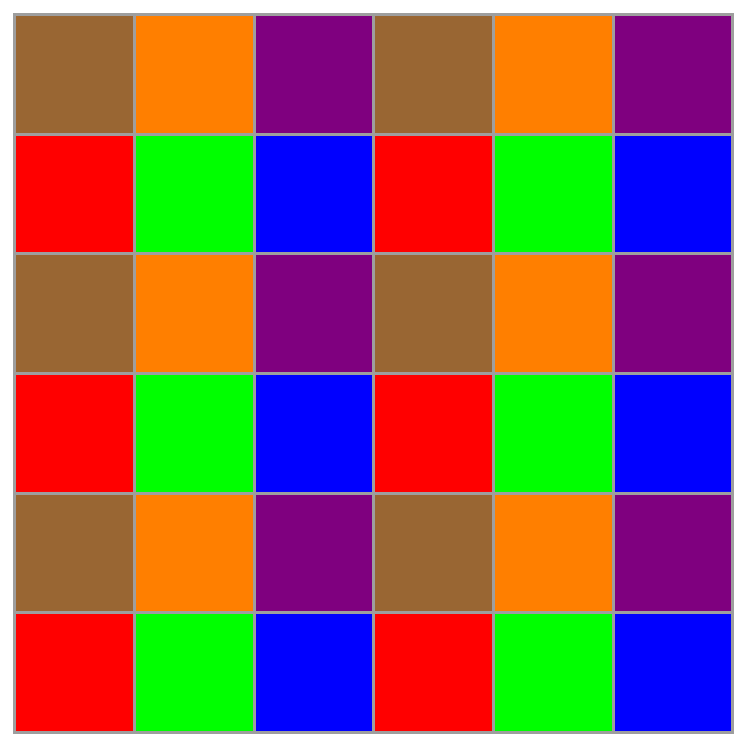
\includegraphics[width=1.0\textwidth]{HL320Block} %\\$\BravCell{3}{2}{0}$ %(b)
            \end{center}\end{minipage}
\]
where the region of symbol plane shown is tiled by 6 repeats of the
$\Mm_{\BravCell{3}{2}{0}}$ \brick, and tile {\color{green}color} = value of
symbol $\Ssym{z}$
\medskip

`stack up' vectors and matrices, vectors as 1\dmn\ arrays,
\beq
\Xx_{\BravCell{3}{2}{0}} =
\left(\begin{array}{c}
 \ssp_{01} \\
 \ssp_{00} \\
  \hline
 \ssp_{11} \\
 \ssp_{10} \\
  \hline
 \ssp_{21} \\
 \ssp_{20} \\
      \end{array}\right)
\,,\qquad
\Mm_{\BravCell{3}{2}{0}} =
\left(\begin{array}{c}
 \Ssym{01} \\
 \Ssym{00} \\
  \hline
 \Ssym{11} \\
 \Ssym{10} \\
  \hline
 \Ssym{21} \\
 \Ssym{20} \\
        \end{array}\right)
\ee{3times2blockVect}
\end{frame} %%%%%%%%%%%%%%%%%%%%%%%%%%%%%%%%%%%%%%%%%%%%%%

\begin{frame}{}
with the $[6\!\times\!6]$ {\jacobianOrb} in block-matrix form
\beq
\jMorb_{\BravCell{3}{2}{0}} =
\left(
\begin{array}{cc|cc|cc}
 -2 s & 2 & 1 & 0 & 1 & 0  \\
 2 & -2 s & 0 & 1 & 0 & 1  \\
  \hline
 1 & 0 & -2 s & 2 & 1 & 0  \\
 0 & 1 & 2 & -2 s & 0 & 1  \\
  \hline
 1 & 0 & 1 & 0 & -2 s & 2  \\
 0 & 1 & 0 & 1 & 2 & -2 s
\end{array}
\right)
\ee{3times2basisVecs}
\end{frame} %%%%%%%%%%%%%%%%%%%%%%%%%%%%%%%%%%%%%%%%%%%%%%


\begin{frame}{summary : orbit stability vs. temporal stability}
\begin{block}{\jacobianOrb}
\(
\jMorb_{ij} =\frac{\delta F[\Xx]_i}{\delta \ssp_j}
\)
stability under {\color{blue}global} perturbation of the whole orbit

\hfill for \cl{} large, a huge $[d\cl{}\!\times\!d\cl{}]$ matrix
\end{block}
\begin{block}{temporal {\jacobianM}}
\(
\jMps%_\Mm
\)
propagates {\color{blue}initial} perturbation $\cl{}$ time steps

\hfill small $[d\!\times\!d]$ matrix
\end{block}
\end{frame}

\begin{frame}{orbit stability vs. temporal stability}
$\jMps$ and $\jMorb$ are {\color{red}always} related by\footfullcite{Hill86}
\begin{block}{Hill's  formula}
\[
|\Det\jMorb_\Mm| = |\det(\matId - \jMps_\Mm)|
%\label{catHillform}
\]
\end{block}
$\jMorb$ is {\color{red}huge}, even $\infty$\dmn\ matrix\\
$\jMps$ is {\color{red}tiny}, few degrees of freedom matrix
\end{frame}

\end{document}
